\section{Korisnički Interfejs}

\subsection{Registracija}
Ekran koji dočekuje sve korisnike sistema pri samom pristupanju je pogled za Registraciju. Sadrži polja za unost teksta kako bi bilo moguće izvršiti registraciju novog korisnika u sistem. Korisnici koji su već dodani u sistem mogu pristupe pogledu za prijavu putem linka u dnu ekrana.


\centerline{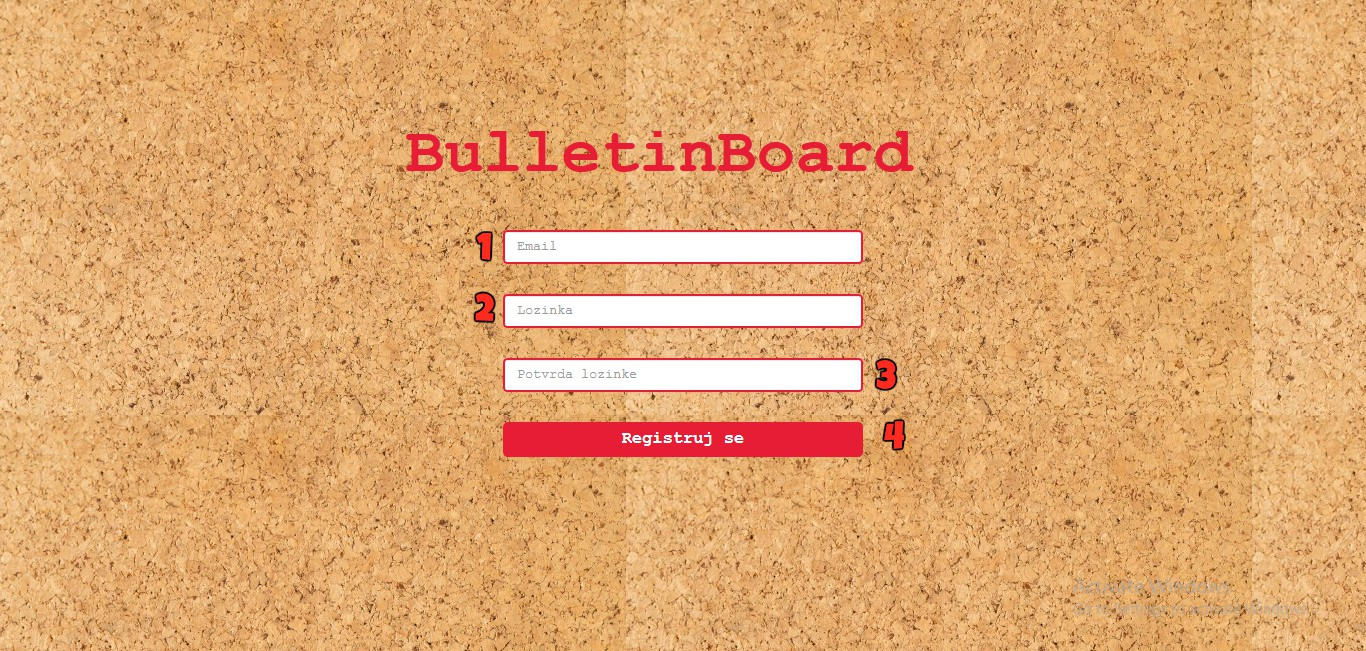
\includegraphics[scale=0.5]{slike/registracija_no.jpg}}
\begin{enumerate}
    \item Tekstualno polje u koje se unosi email za korisnički račun
    \item Tekstualno polje u koje se unosi password za korisnički račun
    \item Tekstualno polje u koje se unosi potvrda passworda za korisnički račun kako ne bi došlo do greške
    \item Dugme kojim se potvrđuje akcija registracije korisničkog računa
\end{enumerate}


\newpage

\subsection{Login}
Korisnici koji su se već registrovali u sistem trebaju se prijaviti prilikom svakog korištenja aplikacije. Na pogledu za prijavu se nalaze polja za unos teksta kako bi se unijeli username i password. Klikom na prijavu se vrši provjera i prijava na sistem.


\centerline{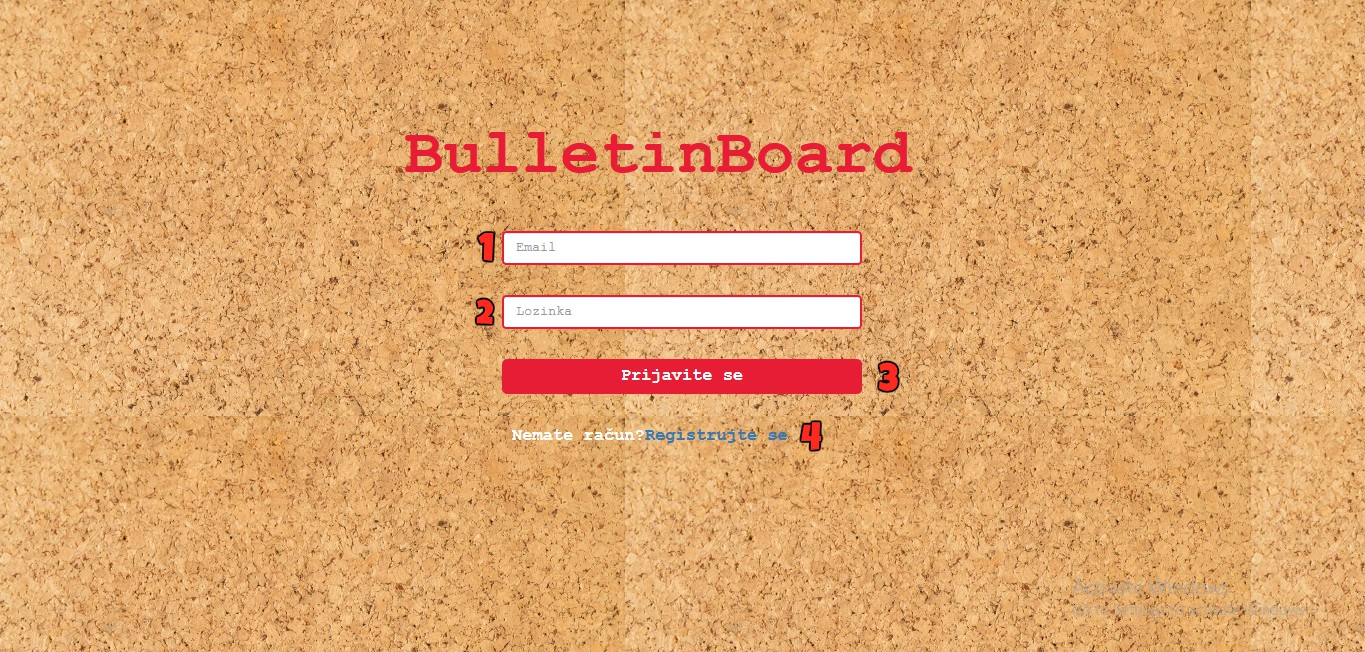
\includegraphics[scale=0.5]{slike/login_no.jpg}}
\begin{enumerate}
    \item Tekstualno polje u koje se unosi email za prijavu u korisnički račun
    \item Tekstualno polje u koje se unosi password za korisnički račun
    \item Dugme kojim se potvrđuje akcija prijave korisnika u sistem
    \item Link za pogled registracije novog korisničkog računa
\end{enumerate}

\newpage

\subsection{Dashboard}
Glavne funkcionalnosti aplikacije se izvršavaju na dashboard pogledu. Korisnici imaju mogućnosti za dodavanje zabilješki, brisanje i modifikaciju istih.


\centerline{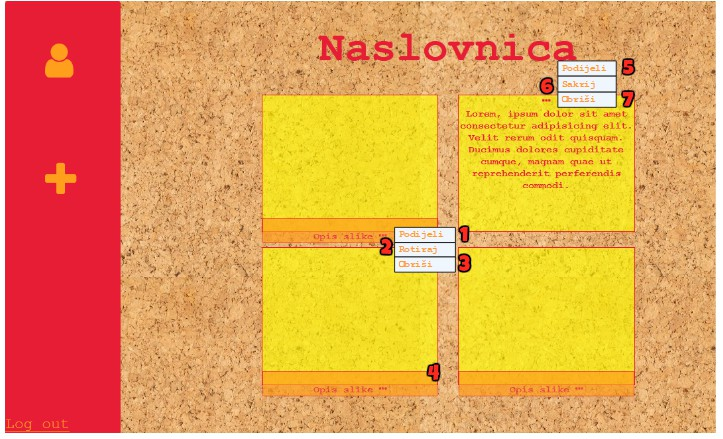
\includegraphics[scale=0.5]{slike/dash_no.jpg}}
\begin{enumerate}
    \item Opcija za dijeljenje slike 
    \item Opcija rotiranja slike
    \item Opcija izbriši sliku
    \item Textarea za dodavanje opisa slike
    \item Opcija za dijeljenje posta
    \item Opcija sakrivanja posta
    \item Opcija izbriši post
\end{enumerate}

\newpage


\subsection{Postavke}
Postavke korisnčkog računa moguće je mijenjati na pogledu za Postavke. Neki od korisničkih podataka koji se mogu mijenjati su prikazani na slici ispod.


\centerline{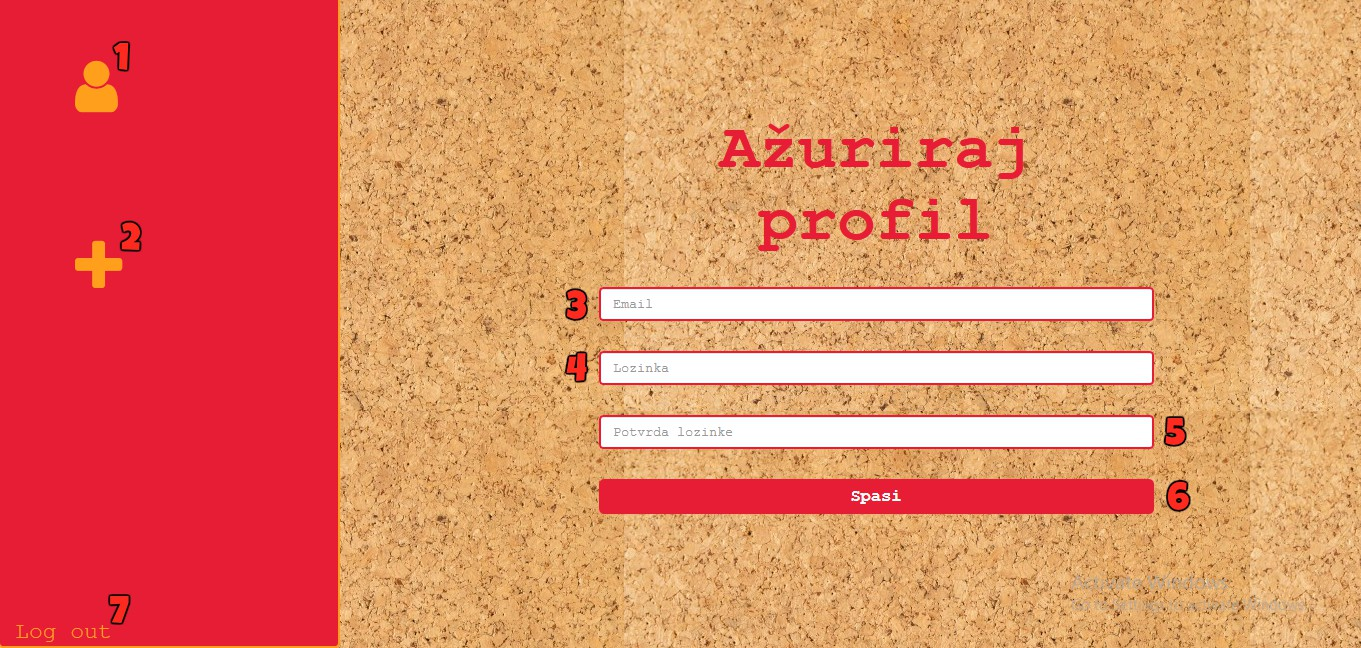
\includegraphics[scale=0.5]{slike/postavke_np.jpg}}
\begin{enumerate}
    \item Dugme koje vodi na korisnički račun
    \item Dugme za dodavanje nove zabilješke
    \item Tekstualno polje u koje se unosi email koji se mijenja
    \item Tekstualno polje u koje se unosi password za korisnički račun
    \item Tekstualno polje za unos potvrde passworda za korisnički račun
    \item Dugme kojim se potvrđuje akcija spašavanja novih postavki korisnika u sistemu
    \item Dugme za odjavljivanje prijavljenog korisnika iz sistema
\end{enumerate}



